\chapter{ALU and ALU Control}
The goal of this lab is to build the ALU and ALU Control modules. These modules can be seen in the context of the datapath by viewing the datapath diagram from a previous lab, Figure~\ref{fig:decode_stage}.  The ALU performs the arithmetic and logical operations, and the ALU Control module determines which operation should be performed by the ALU.  During this lab, we will not put these modules together.  Instead, they will be tested independently of each other.
\section{ALU}
The ALU has three inputs:
\begin{enumerate}
	\item a\_in - the first input operand
	\item b\_in - the second input operand
	\item alu\_control - control signal used to tell the ALU what operation to perform
\end{enumerate}
The ALU has two outputs:
\begin{enumerate}
	\item alu\_result - the result of the arithmetic/logic operation
	\item zero - a flag indicating whether alu\_result is zero
\end{enumerate}  
Figure~\ref{fig:alu_control_table} identifies the operation that corresponds to the alu\_ctrl value.  Note that we will not be implementing NOR, even though it is listed in the table.  You should use a case statement to evaluate the alu\_control bits to determine which ALU operation to perform.  For each operation, you do not have to do anything fancy.  You just need to use the math capability that verilog provides to make the calculation.  To make the code readable, you must give the the ALU control bits names in the definitions.vh file, and you should use these in your cases.  Please use the following names for your macros in defintions.vh:
\begin{enumerate}
	\item ALU\_AND
	\item ALU\_ORR
	\item ALU\_ADD
	\item ALU\_SUB
	\item ALU\_PASS
\end{enumerate}
Also, don't forget to make a default case, which is needed to actually wire this up.  Please use AND for the default case.

One last thing to note is the generation of the zero flag.  The zero flag is determine by simply evaluating the alu\_result.  There are several ways to handle this, but this is the easiest way to handle it.  In Verilog (like C), the statement $(y==0)$ is an operation with a boolean output.  You can thus say $x=(y==0);$ to assign $x$ to be the boolean value that $(y==0)$ produced.  The statement $x=(y==0);$ is realizable as a digital comparator with $y$ and $0$ as inputs and $x$ as the single bit output.  Please note that you will not have signals called $x$ and $y$.  I just used these to explain the concept.

\begin{figure}
	\caption{ALU Control Values}\label{fig:alu_control_table}
	\begin{center}
		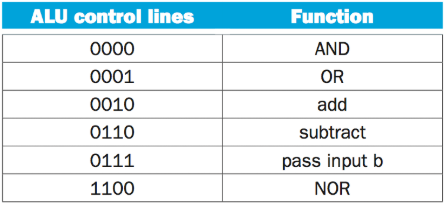
\includegraphics[width=2.75in]{../images/alu_control_table.png}
	\end{center}
\end{figure} 

\section{ALU Control}
The ALU Control module has two inputs:
\begin{enumerate}
	\item alu\_op - 2 bit signal giving incomplete information about what ALU operation should be performed
	\item opcode - the opcode of the instruction
\end{enumerate}
The ALU Control module has one output:
\begin{enumerate}
	\item alu\_control - control signal used to tell the ALU what operation to perform
\end{enumerate}
You have already defined the ALUOp macros in definitions.vh when you created the control module.  You have also already defined the ALU Control macros in definitions.vh in the previous section.  And you have macros defined for instruction opcodes. Please use these macros when creating the ALU Control module.

Figure~\ref{fig:alu_control_table} identifies the operation that corresponds to the alu\_ctrl value.  This module can be implemented multiple ways, but we want to use the most efficient way possible.  The most efficient method is to use a casex statement to evaluate the alu\_op signal, utilizing the information in Figure~\ref{fig:alu_op_opcode_table}.  alu\_op will provide all information necessary for D-Type and CB-Type instructions.  For R-Type instructions, you should use the bits of the opcode to set the alu\_ctrl value.  When evaluating Figure~\ref{fig:alu_op_opcode_table} for R-Type instructions, certain bits of the instruction correspond to alu\_ctrl bits.  The magic decoder ring is listed below.  Please note that the numbering system for the instruction bits includes the entire instruction, whereas you will just have the opcode to work with.  Therefore, you will need to adjust the numbering to account for your 11-bit opcode.
\begin{enumerate}
	\item ALU Ctrl [3] = 0
	\item ALU Ctrl [2] = I[30]
	\item ALU Ctrl [1] = I[24]
	\item ALU Ctrl [0] = I[29]
\end{enumerate} 

Please use AND as the default case.  For the B instruction, the ALU Op should be 00 from your control module.  Since 00 is also the ALU Op for LDUR and STUR (which have ALU Control value of ADD), you can just allow the B instruction to also set ALU Control to ADD.

\begin{figure}
	\caption{ALU Op Table}\label{fig:alu_op_opcode_table}
	\begin{center}
		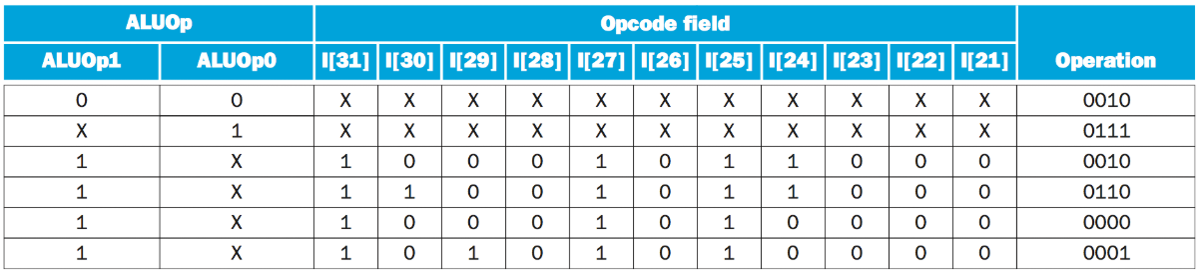
\includegraphics[width=4.75in]{../images/alu_op_opcode_table.png}
	\end{center}
\end{figure} 

\section{Your Assignment}

You are to:
\begin{enumerate}
\item Create the ALU module.
\item Verify that your ALU module works correctly by running it against the provided test bench.
\item Create an ALU Control module.
\item Verify that your ALU module works correctly by running it against the provided test bench.
\item Rather than writing a lab report, please produce a landscape mode PDF file called Lab8\_lastname.pdf that includes (in this order):
\begin{enumerate}
	\item Your name and the lab number.
	\item A snip of the Simulation Results for the each test bench.  Please show instructions in hex, opcodes and control signals in binary and everything else in signed decimal.  
	\item For each test bench, copy and paste the entire log from BEGIN TEST RESULTS to END TEST RESULTS into your file.	
\end{enumerate}
\item Upload Lab8\_lastname.pdf file to Canvas.
\item Zip up your ARM-Lab directory and submit it on Canvas as well.  Please make sure that you give me the ARM-Lab directory rather than the ARM-Project directory.  I do not want the project files in the ARM-Project directory.  Before you submit your zip file, extract the file and make sure that the top-level directory is called ARM-Lab and that the lower level directories like code, manual, etc are directly beneath ARM-Lab in the directory structure.  I will extract your zip file and run your code against my correct testbench to verify that your code and testbench work correctly, and it is critical that everyone's directory structure is consistent.
\end{enumerate} 